\documentclass[12pt,a4paper]{article}
\usepackage[utf8]{inputenc}%Para Tildes y ñ%
\usepackage[spanish]{babel}
\usepackage{amsmath}
\usepackage{amsfonts}
\usepackage{amssymb}
\usepackage{adjustbox}
\usepackage{graphicx} 
\usepackage{pdfpages} %para importar paginas de un pdf
\usepackage{booktabs}
\usepackage[bookmarks = true, colorlinks=true, linkcolor = black, citecolor = green, menucolor = black, urlcolor = black]{hyperref} 
\usepackage[left=2cm,right=2cm,top=2cm,bottom=2cm]{geometry} 
\usepackage{multirow}
\addto\captionsspanish{\renewcommand{\listtablename}{Índice de tablas}}		% Cambiar nombre a lista de tablas   
\addto\captionsspanish{\renewcommand{\tablename}{Tabla}}					% Cambiar nombre a tablas
\usepackage{float}		% Para ubicar las tablas y figuras justo después del texto
\usepackage{pdfpages}
\usepackage{enumerate}%listas y viñetas
\usepackage{svg}
\usepackage{siunitx}
\usepackage{comment}
\usepackage{mathtools}
\usepackage[shortlabels]{enumitem}
\usepackage{subcaption}
\DeclarePairedDelimiter\abs{\lvert}{\rvert}%
\DeclarePairedDelimiter\norm{\lVert}{\rVert}%

\makeatletter
\let\oldabs\abs
\def\abs{\@ifstar{\oldabs}{\oldabs*}}
%
\let\oldnorm\norm
\def\norm{\@ifstar{\oldnorm}{\oldnorm*}}
\makeatother


\usepackage{circuitikz}
%\usepackage{subfig}
\usepackage{listings}
\usepackage{verbatimbox}
\usepackage{multicol}
\usepackage{xcolor}
\usepackage{verbatimbox}

%\setcounter{secnumdepth}{0} % ///////////////////////////////////////////// Para que los \section no tenga numeros
\newfloat{Resultado}
\captionsetup{Resultado}
%New colors defined below
\definecolor{codegreen}{rgb}{0,0.6,0}
\definecolor{codegray}{rgb}{0.5,0.5,0.5}
\definecolor{codepurple}{rgb}{0.58,0,0.82}
\definecolor{backcolour}{rgb}{0.95,0.95,0.92}

%Code listing style named "mystyle"
\lstdefinestyle{mystyle}{
  backgroundcolor=\color{backcolour}, commentstyle=\color{codegreen},
  keywordstyle=\color{magenta},
  numberstyle=\tiny\color{codegray},
  stringstyle=\color{codepurple},
  basicstyle=\ttfamily\footnotesize,
  breakatwhitespace=false,         
  breaklines=true,                 
  captionpos=b,                    
  keepspaces=true,                 
  numbers=left,                    
  numbersep=5pt,                  
  showspaces=false,                
  showstringspaces=false,
  showtabs=false,                  
  tabsize=2
}



\title{Universidad de Costa Rica\\{\small Facultad de Ingeniería \\Escuela de Ingeniería Eléctrica\\IE0624 - Laboratorio de Microcontroladores \\\vspace*{2in}}\\ \textbf{Laboratorio 4 - STM32: GPIO, ADC, comunicaciones, Iot}  \vspace*{0.55in}\\ 
\author{Andrés Artavia Solano - B90789 \\ Mario Navarro Bejarano - B75398  \vspace*{3.0in}}\\ Prof. MSc. Marco Villalta Fallas
\vspace*{0.8in}}

\date{II - 2024} 
\begin{document} 

\maketitle  
\thispagestyle{empty}%%no numerar la portada
\renewcommand{\thepage}{\roman{page}}
\newpage
\tableofcontents
%\listoffigures 
\newpage
%\listoftables  
%\newpage
%%%%%%%%%%  
\renewcommand{\thepage}{\arabic{page}} 
\setcounter{page}{1}

\section{Introducción}
En este laboratorio se busca desarrollar un sismógrafo básico utilizando la placa STM32F429 Discovery Kit y la biblioteca libopencm3, aprovechando la capacidad del giroscopio para detectar movimientos en los ejes X, Y, Z. Este proyecto representa una aplicación práctica del uso de microcontroladores en sistemas de monitoreo sísmico, permitiendo adquirir habilidades en la integración de sensores, manejo de periféricos y transmisión de datos en un entorno de Internet de las Cosas (IoT).
El diseño del sismógrafo se enfoca en capturar las variaciones de los ejes del giroscopio, indicando potenciales eventos sísmicos. A través de un sistema de comunicación USART/USB, se habilitará la transmisión de los datos a una computadora para posteriormente transmitir los datos a una plataforma IoT. Además, se integrará un sistema de monitoreo del nivel de batería, crucial para asegurar la operación continua del dispositivo.
El principal objetivo de este laboratorio es diseñar e implementar un sistema de monitoreo sísmico básico utilizando la placa STM32F429 Discovery Kit, con la finalidad de capturar movimientos en los ejes X, Y, Z mediante el giroscopio incorporado, simulando las funciones de un sismógrafo. Además, se busca proporcionar al usuario la capacidad de habilitar o deshabilitar la transmisión de datos mediante un switch físico, permitiendo controlar la comunicación serial a conveniencia.
El sistema incluirá un LED indicador, que parpadeará cuando la transmisión USART esté habilitada. También se implementará un mecanismo de monitoreo del nivel de batería, en caso de que la tensión descienda por debajo del límite de operación seguro (7V), se encenderá un LED de alarma y se enviará una notificación de batería baja al dashboard IoT en ThingsBoard.
También se planea desplegar en la pantalla LCD los valores del giroscopio en los tres ejes, el nivel de batería, y el estado de la comunicación USART/USB. Finalmente, se desarrollará un script en Python que permitirá transmitir la información del giroscopio y el estado de la batería al dashboard de ThingsBoard, donde los datos podrán ser visualizados de forma intuitiva mediante widgets. 

\vspace{1cm}\\
\textit{Nota: El código fuente se puede encontrar en la rama  ``main" del repositorio, en la carpeta ``lab4". \url{https://github.com/artavias/IE0624/tree/main}}

\newpage
\section{Nota Teórica}

A continuación se muestra un diagrama del diseño general de la placa:
\begin{figure}[H]
    \centering
    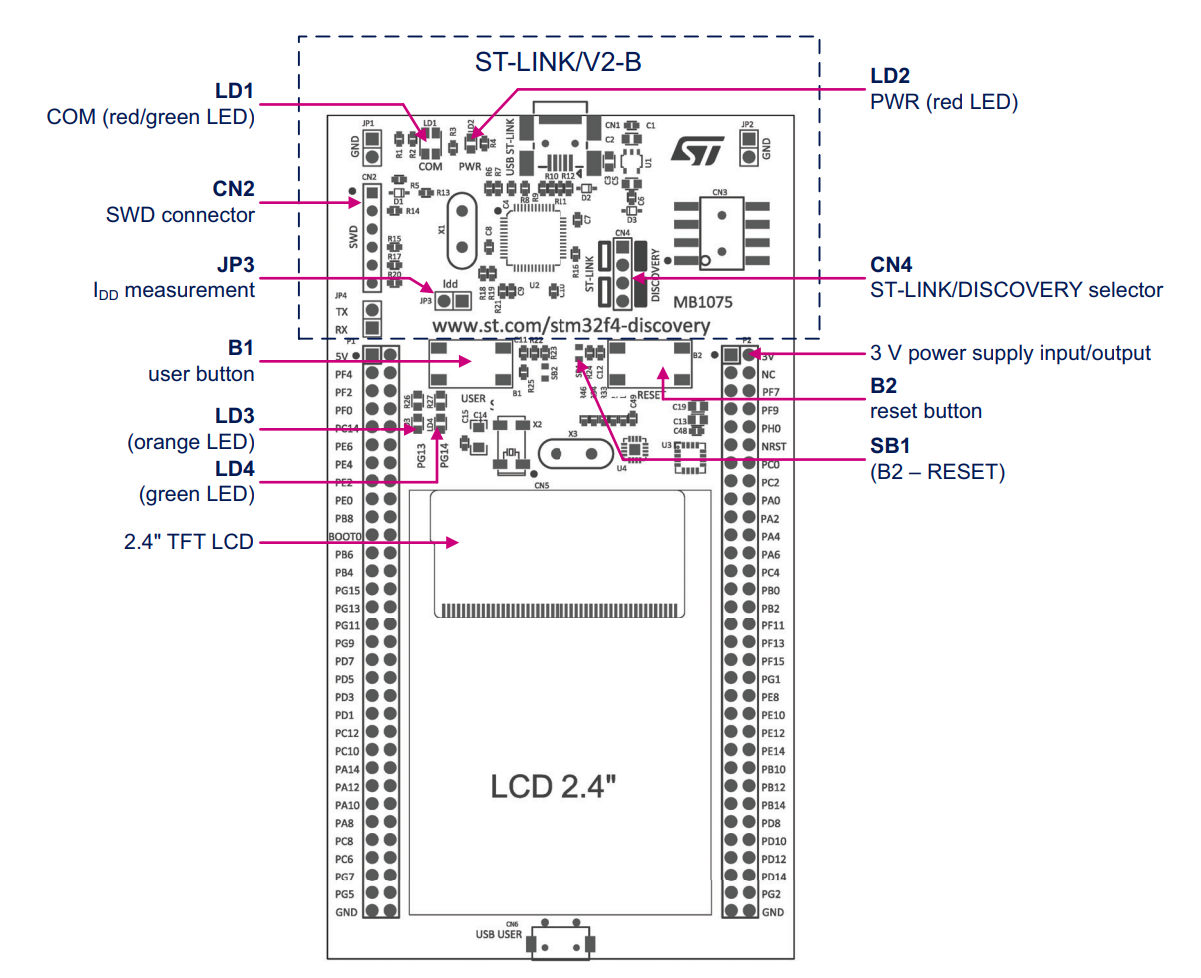
\includegraphics[scale=.5]{Imagenes/layout.png}
    \caption{Diseño general del STM32F429i Discovery Kit \cite{discovery}}
    \label{fig:diag_general}
\end{figure}

\subsection{Componentes empleados.}
La siguiente tabla detalla los componentes y la cantidad utilizada.
\begin{center}
    \begin{tabular}{|c|c|}
        \hline
         Componente & Cantidad\\ \hline
         STM32F429i Discovery Kit & 1\\
         Bateria 9V & 1 \\
         Resistencia 10k$\Omega$ & 2 \\
         Resistencia 2.2k$\Omega$ & 1 \\ \hline
    \end{tabular}
\end{center}

\subsection{STM32F429ZI}
La siguiente datos de la placa STM32F429 Discovery kit fueron tomados de la hoja de datos oficial del fabricante \cite{discovery}.
La placa STM32F429 Discovery kit se basa en el microcontrolador STM32F429ZI, el cual es un microcontrolador de alto rendimiento de la serie STM32F4 desarrollado por STMicroelectronics, basado en el núcleo ARM Cortex-M4. Este procesador está diseñado para aplicaciones de tiempo real que requieren cálculos intensivos y alto control sobre periféricos. A continuación, se detalla su arquitectura, características clave del procesador, y el uso de registros.
El procesador ARM Cortex-M4 integrado en el STM32F429ZI opera a una frecuencia de 180 MHz. Este procesador incorpora una Unidad de Punto Flotante (FPU) compatible con el estándar IEEE 754, lo que permite realizar operaciones de punto flotante de forma rápida y eficiente. Además, incluye una caché de instrucciones y datos (I/D), que optimiza la velocidad de acceso a memoria y minimiza las latencias durante la ejecución del código.
El Cortex-M4 soporta procesamiento digital de señales (DSP), incorporando instrucciones SIMD (Single Instruction Multiple Data), que mejoran el rendimiento en algoritmos matemáticos, como filtros y procesamiento de señales, aumentando la eficiencia del sistema. Ofrece un sistema de gestión de interrupciones capaz de manejar hasta 240 interrupciones con 16 niveles de prioridad. Estas interrupciones son gestionadas por el NVIC (Nested Vectored Interrupt Controller), asegurando respuestas rápidas y eficientes a eventos de hardware software críticos.
El microcontrolador dispone de 2 MB de memoria Flash interna, utilizada para almacenar el firmware y las aplicaciones críticas. Esta memoria permite múltiples ciclos de lectura y escritura, garantizando la estabilidad del sistema durante las actualizaciones. Además, cuenta con 256 KB de SRAM interna para la ejecución de tareas en tiempo real. Para aplicaciones que requieren un manejo intensivo de datos, como el procesamiento de señales, el sistema puede hacer uso de una memoria externa SDRAM de 64 Mbits, útil para almacenamiento temporal y creación de buffers.
El STM32F429ZI ofrece varios puertos GPIO (General Purpose I/O), los cuales se configuran a través de registros específicos para definir su modo de operación, ya sea como entrada, salida, función alternativa o analógica.
El microcontrolador dispone de hasta 14 temporizadores, algunos de ellos con funciones avanzadas como la generación de PWM (Pulse Width Modulation). Cada temporizador se gestiona mediante los registros de control de temporizadores.

\subsection{Giroscopio y pantalla LCD}
La interfaz SPI permite la comunicación entre el microcontrolador y el giroscopio MEMS I3G4250D.
El giroscopio MEMS I3G4250D integrado en la placa es un sensor de movimiento de tres ejes que permite medir la velocidad angular en rangos ajustables de ±245, ±500 o ±2000 grados por segundo (dps), lo que lo hace adecuado para aplicaciones de monitoreo de vibraciones y detección de movimientos sísmicos. Este giroscopio cuenta con una interfaz de salida digital compatible con SPI e I2C, lo que facilita su integración con el microcontrolador y permite la captura eficiente de datos en tiempo real. Además, el I3G4250D incluye un filtro pasa bajos configurable que mejora la precisión en la medición de cambios de orientación y detecta variaciones sutiles en el movimiento en los ejes X, Y y Z.
La pantalla LCD TFT integrada es de 2.4 pulgadas con una resolución QVGA de 240 x 320 píxeles y es capaz de mostrar hasta 262,000 colores. Es controlada mediante un controlador ILI9341 a través de un protocolo RGB, esta pantalla facilita la visualización de información como el nivel de batería, los datos de los ejes del giroscopio y el estado de la comunicación USART/USB. Además, su bajo consumo de energía y compatibilidad con voltajes típicos de 2.8 V la hacen ideal para aplicaciones en sistemas portátiles.

\subsection{ThingsBoard}
ThingsBoard es una plataforma de Internet de las Cosas (IoT) de código abierto que permite recopilar, procesar y visualizar datos en tiempo real desde dispositivos y sensores conectados. Facilita la administración remota y el monitoreo de dispositivos IoT, ofreciendo herramientas avanzadas para crear visualizaciones interactivas, analizar datos y generar alertas según condiciones específicas.
Entre sus características principales se encuentra la gestión de dispositivos, que permite registrar y controlar dispositivos IoT de manera eficiente. Cada dispositivo puede configurarse para enviar datos en intervalos regulares o cuando ocurren eventos específicos, utilizando protocolos de comunicación como MQTT, HTTP y CoAP, lo cual permite una fácil integración con diversos dispositivos.
ThingsBoard también permite el procesamiento y almacenamiento de datos a gran escala en tiempo real, aplicando reglas de procesamiento para ejecutar acciones basadas en eventos, como activar alertas o enviar datos a servicios en la nube cuando se cumplen condiciones específicas. Permite crear dashboards personalizables con widgets interactivos como gráficos de líneas, medidores, tablas y mapas, facilitando el análisis y la monitorización de datos en tiempo real.
La plataforma permite configurar alertas y notificaciones basadas en reglas definidas por el usuario, ideal para aplicaciones que requieren alertas inmediatas en situaciones críticas, como baja batería o detección de actividad sísmica. Estas notificaciones pueden enviarse por correo electrónico o integrarse con otros sistemas de mensajería en tiempo real.
Diseñada para aplicaciones de cualquier escala, ThingsBoard es altamente escalable y cuenta con características de seguridad avanzadas que incluyen autenticación de dispositivos, control de acceso basado en roles y cifrado de datos. \cite{things}
En este laboratorio, ThingsBoard se utilizará para recibir y visualizar datos del giroscopio y el nivel de batería de la placa STM32F429 Discovery Kit. Un script en Python enviará estos datos a la plataforma, representándolos en un dashboard interactivo para observar en tiempo real las variaciones de movimiento y el estado de la energía. Además, las alertas configuradas en ThingsBoard enviarán notificaciones en caso de batería baja, garantizando una respuesta rápida ante condiciones críticas.




\newpage
\section{Desarrollo}
\subsection{Lectura de Giroscopio}
El primer punto que se debe resolver es realizar la lectura de los valores en los ejes X, Y y Z del giroscopio. Para realizar esta sección, se utilizó parte del código que se proporciona por los ejemplos de libopemcm3, esto para funciones no relevantes para los objetivos de este laboratorio, como configurar el reloj del sistema por ejemplo.\\
En la figura \ref{codig1} se muestra el código utilizado para configurar los pines y el SPI5, estos son los elementos necesarios para comunicarse con el giroscopio. Primero se configuran los puertos GPIO, como salidas, así como las frecuencias, luego se configuran los registros SPI5 para habilitarlo a funcionar en modo maestro, dados los parámetros de funcionamiento de la interfaz SPI5 del giroscopio. Es importante mencionar que el orden en el que se llaman estas funciones es el orden que se indica en las diapositivas del curso.

\begin{figure}[H]
    \centering
    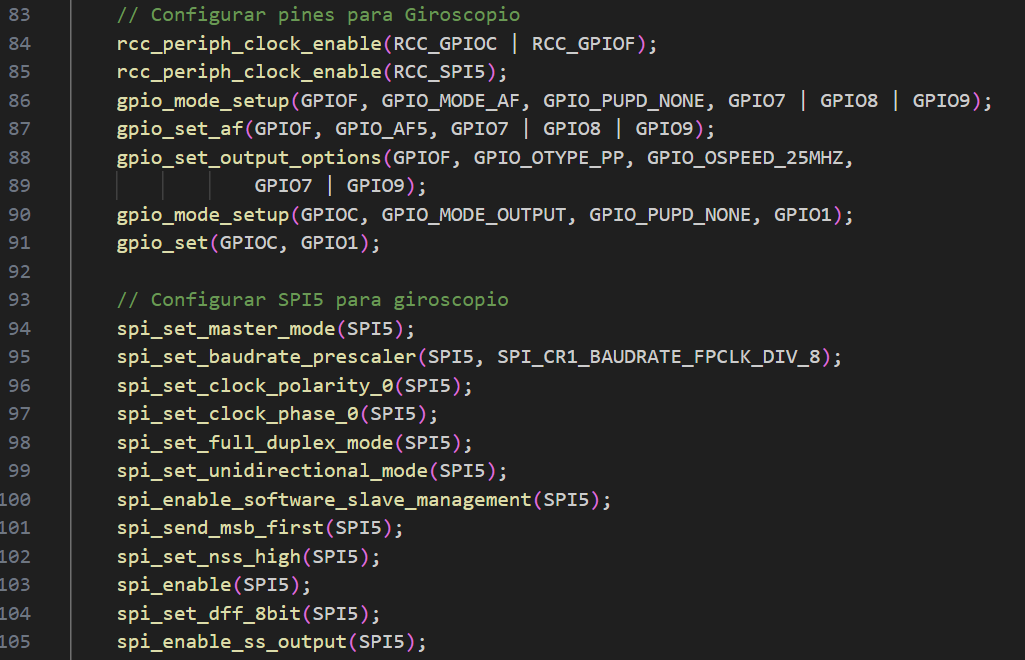
\includegraphics[scale=.5]{Imagenes/codig1.png}
    \caption{Codigo para configurar comunicación con SPI5}
    \label{codig1}
\end{figure}

Luego de realizar estas configuraciones, se pueden configurar los registros del giroscopio y proceder a leer los registros correspondientes a los valores X, Y y Z, tal como se muestra en la figura \ref{codig2}

\begin{figure}[H]
    \centering
    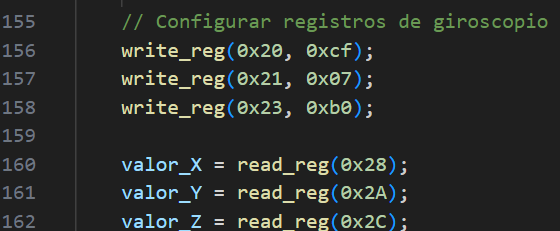
\includegraphics[scale=.5]{Imagenes/codig2.png}
    \caption{Escritura y lectura de registros del giroscopio.}
    \label{codig2}
\end{figure}


Nota importante: Se realizaron múltiples intentos de establecer la comunicación con el giroscopio, desde modificaciones en la configuración de SPI5, simular las comunicaciones SPI5 manualmente, probar ejemplos proporcionados hasta probar codigo proporcionado por compañeros del curso a los cuales sí les funcionaba, sin embargo, no fue posible obtener datos fuera de un constante valor de 0, por ello se llegó a la conclusión de que puede existir algún daño físico en la placa, lo que impide la comunicación con el giroscopio, o que el daño existe en sí en el giroscopio.\\
Para compensar esta carencia, se comentó esta sección del código (en teoría el código sigue siendo funcional y se podría utilizar en una placa en buen estado) y se agregaron unos contadores que simulan el cambio en los valores que proporcionaría el giroscopio. Más adelante en la sección de resultados se mostrará este funcionamiento.

\subsection{LED's, botón y ADC}
Para realizar la configuración de los leds que se usarán para indicar que la tensión de la batería está baja, que la comunicación USART está activada, del botón para habilitar esta comunicación y del convertidor analógico digital, se realizó un proceso de configuración muy similar al que se utilizó para configurar la comunicación con el giroscopio, con la diferencia del cambio de los pines. Así que para evitar extender este reporte, se omite agregar esta sección del código.\\
Fuera de la configuración, en la figura \ref{codig3} se muestra el codigo con la lógica para controlar estas funciones. En las lineas 192-164 se muestra la lógica para encender el led cuando se presiona el botón, esta información se utiliza también para habilitar la comunicación USART. En las lineas 165-167 se muestra el código que se encarga de leer la información sobre la tensión de la batería. En este caso esta información muestra la tensión en mili-volts, para aprovechar la precisión del ADC. Finalmente en las lineas 169-177 se muestra la lógica que se utiliza para encender y apagar el led de color rojo, esta función se activa cuando la tensión es inferior a 7.5V, por lo que se acerca a la tensión de peligro de 7V.

\begin{figure}[H]
    \centering
    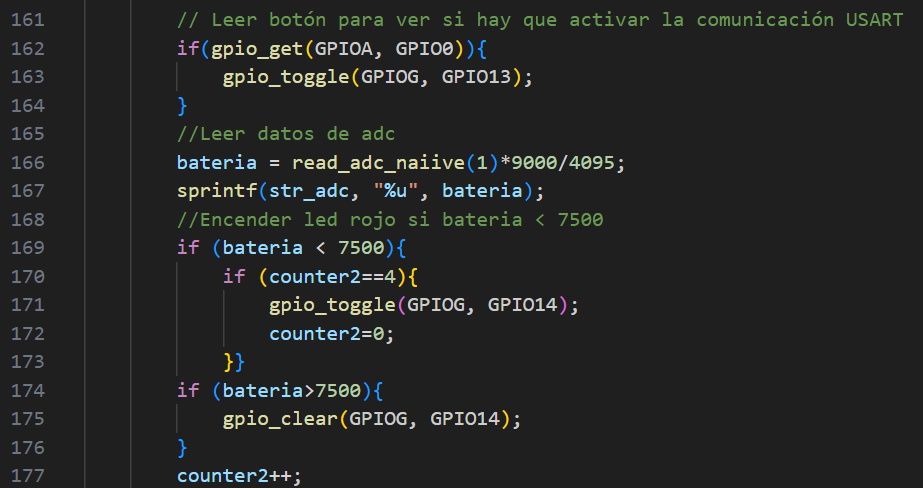
\includegraphics[scale=.6]{Imagenes/codig3.png}
    \caption{Código para controlar leds y comunicación.}
    \label{codig3}
\end{figure}

\subsection{Nivel de batería}
Para poder medir el nivel de la batería de 9V se puede utilizar un ADC de 12 bits incluido en la placa, pero primero es necesario condicionar la tensión de la batería a un rango seguro para la placa de 5V. Para esto se construyó un divisor de tensión utilizando las resistencias disponibles en la bodega, se opto por utilizar dos resistencias de 10k$\Omega$ y una de 2.2k$\Omega$. El siguiente diagrama muestra el circuito construido:
\begin{figure}[H]
    \centering
    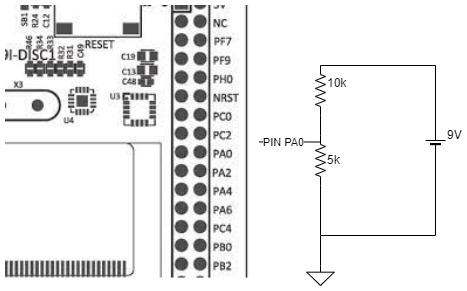
\includegraphics[scale=.7]{Imagenes/bateria (3).jpg}
    \caption{Esquemático del divisor de tensión. Diagrama de la placa tomado de \cite{discovery}}
    \label{fig:divisor}
\end{figure}

Como se muestra en la figura \ref{fig:divisor} la tensión de la batería pasaría a condicionarse a un nivel en donde la tensión máxima, es decir cuando la batería se encuentre a 9V, viene dado por:
\begin{equation}
    V_{out} = 9 \cdot \frac{5k}{10k+5k} = 3V
\end{equation}

De esta manera podemos conectar el pin PA0 al divisor de tensión de manera segura sin sobrepasar los limites de la placa. 

Ahora utilizando el ADC de 12 bits de la placa se configura para leer el nivel de tensión del pin PA1 y se obtiene un valor periódicamente que va de 0 a 4095. Este rango del ADC corresponde a un rango de tensión en el pin de 0 a 3.3V pero como calculamos anteriormente, el máximo valor de tensión que puede alcanzar a medirse en el pin es de 3V, gracias al circuito de acondicionamiento. Si realizamos un calculo rápido podemos ver que este valor corresponde a 3723 en el rango del ADC:
\begin{equation}
    3V \cdot \frac{4095}{5} = 3722.72
\end{equation}

El ADC en este caso nos daria mediciones en un rango 
de 0 a 3723, tomando esto en cuenta se puede mapear el valor a un rango de 0 a 9V nuevamente para obtener finalmente el nivel de tensión de la batería. Para mapear el valor a este nuevo rango simplemente se multiplica por 9 y se divide entre 3723 el valor obtenido del ADC.

En nuestro caso no fue posible encontrar un adaptador adecuado para conectar la batería y realizar el circuito, pero el código necesario para medir la tensión de la batería utilizando el divisor de tensión diseñado se puede encontrar en el repositorio del laboratorio. 

\subsection{Dashboard en ThingsBoard}
El primer paso para enviar los datos al dashboard de ThingsBoard es leer los datos enviados por la placa, para esto se establece conexión creando un objeto de tipo Serial() con el puerto serial que en este caso corresponde a ‘COM14’ con una tasa de 115200 baudios. 
Para enviar los datos al dashboard de ThingsBoard primero fue necesario agregar un dispositivo y generar un token necesario para realizar la conexión al host. Luego es necesario crear un objeto de tipo ‘mqtt.Client()’ y especificarle el host y el puerto para iniciar un loop infinito en donde se leen los datos del puerto serial y se ‘parsean’, es decir que se ordenan y se extraen los datos de los ejes, así como el nivel da la batería. Estos datos se utilizan para formar un diccionario el cual se envía como un objeto de tipo ‘json’ mediante la función ‘publish’.

A continuación se muestra el código utilizado: 
\begin{figure}[H]
    \centering
    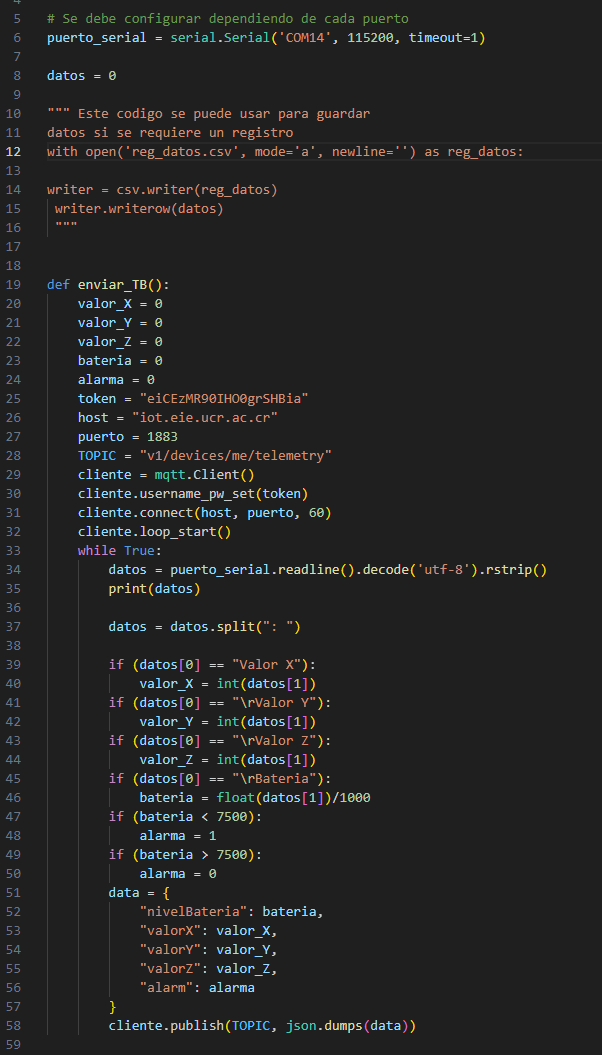
\includegraphics[scale=.7]{Imagenes/python.png}
    \caption{Script para leer y enviar datos a ThingsBoard}
    \label{fig:py}
\end{figure}



\newpage
\section{Análisis de los resultados}
A continuación se muestran capturas del funcionamiento del código implementado.

\begin{figure}[H]
    \centering
    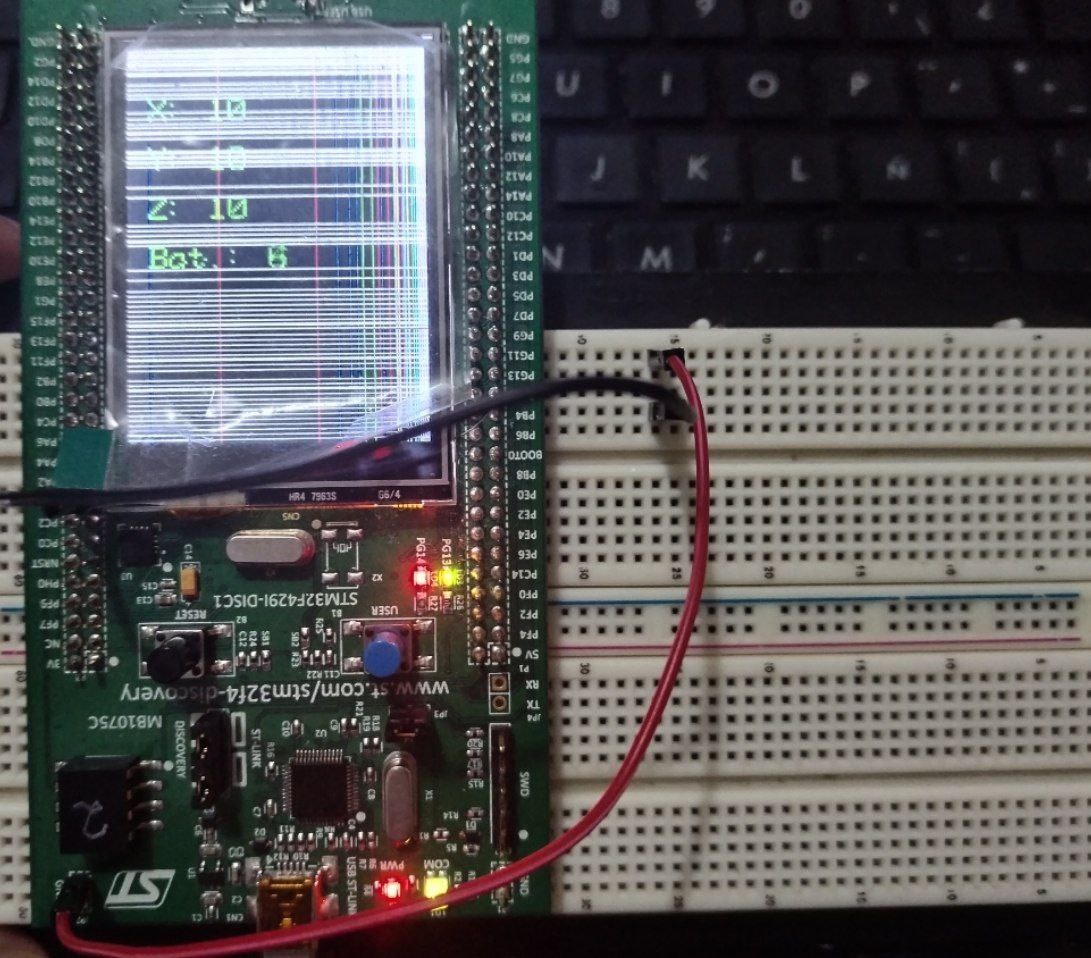
\includegraphics[scale=.3]{Imagenes/codig4.png}
    \caption{Muestra de información en pantalla.}
    \label{codig4}
\end{figure}

En la figura \ref{codig4} se muestra el funcionamiento de la placa, se pueden observar las siguientes características:
\begin{itemize}
    \item En pantalla se muestra el valor del giroscopio (simulado) en los tres ejes. No es claramente visible debido al daño que presenta la pantalla.
    \item Se muestra encendido el led verde, este indica que la comunicación USART se encuentra activa. Cuando se presiona el botón la comunicación se desactiva y el led se apaga.
    \item  Se puede observar el led rojo encendido. Este led parpadea indicando que la batería tiene un nivel de tensión inferior a 7.5V, esto también se puede observar en la pantalla, que indica una medida de 5mV, casi cero. esto porque el pin ADC se conectó con jumpers al pin GND. Si este pin se conecta a tensión, el valor en pantalla indica 9000mV, es decir, indica que la batería está cargada y por lo tanto el led rojo deja de parpadear.
\end{itemize}
\begin{figure}[H]
    \centering
    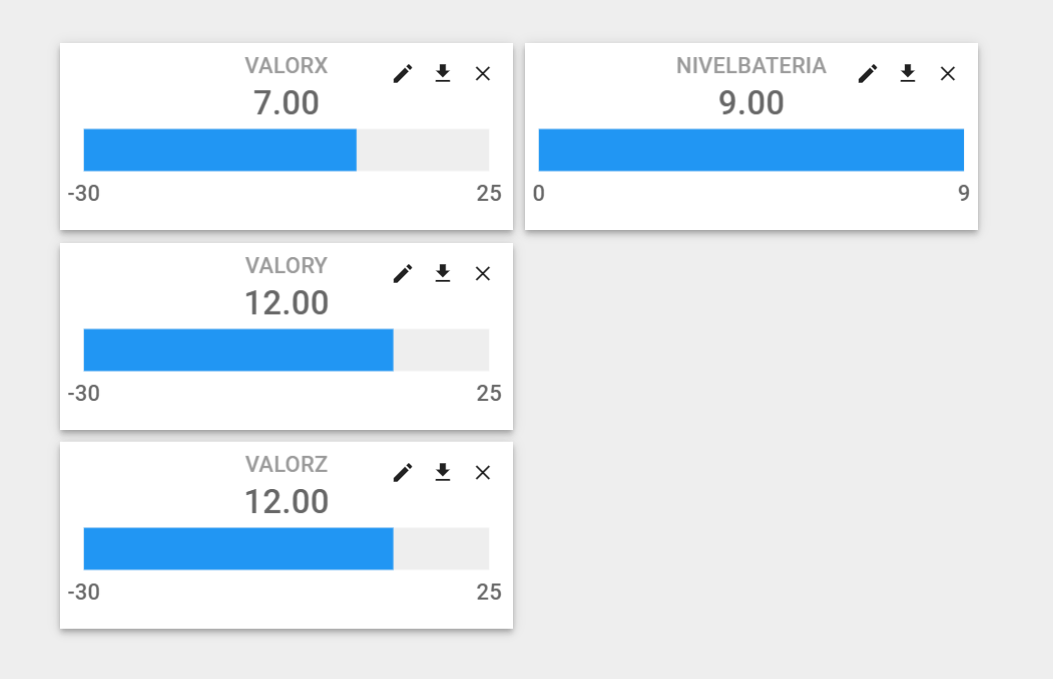
\includegraphics[scale=.3]{Imagenes/TB.png}
    \caption{Muestra del dashboard en thingsboard al que se conecta la placa}
    \label{TB}
\end{figure}
En la figura \ref{TB} se muestra el dashboard de thingsboard. Se puede observar en la columna de la izquierda que se muestran los valores de los 3 ejes. En este caso se están simulando valores de 7, 12 y 12 para X, Y y Z respectivamente. A la derecha se observa el indicador de la batería, en este caso el ADC se conectó a tensión máxima, por lo que se indica una tensión de 9V.







\newpage
\section{Conclusiones}
En este laboratorio, el objetivo era implementar un sistema de monitoreo basado en la lectura de datos del giroscopio en la placa STM32F429 Discovery Kit y su transmisión a la plataforma IoT ThingsBoard. Sin embargo, debido a un fallo en el giroscopio, no fue posible obtener datos reales de los ejes X, Y y Z. Para completar el proyecto, se optó por simular los datos del giroscopio, lo que permitió probar la funcionalidad de adquisición, procesamiento y envío de información a ThingsBoard, cumpliendo así los objetivos de transmisión y visualización en tiempo real.

A pesar de la limitación técnica con el sensor, la simulación de los datos fue útil para verificar el funcionamiento del sistema de comunicación y el correcto envío de la información al dashboard de ThingsBoard. Esta simulación permitió observar en tiempo real cómo los valores del giroscopio (aunque simulados) se desplegaban en la plataforma, confirmando que el sistema era capaz de transmitir datos de manera eficiente y que el dashboard estaba correctamente configurado para recibir y visualizar la información.

La transmisión de datos vía USART se configuró para enviar la información simulada del giroscopio y el estado de la batería. La comunicación mediante USART fue exitosa, ya que el sistema transmitió datos a ThingsBoard en tiempo real, donde se visualizaron correctamente en el dashboard. Adicionalmente, se implementó un control de habilitación mediante un switch físico, lo cual facilitó la activación y desactivación de la transmisión. 

Para mejorar futuros laboratorios, se recomienda comenzar con una verificación previa de los componentes, asegurando que el giroscopio y otros sensores funcionen adecuadamente antes de iniciar la implementación. Ante posibles fallas, sería útil contar con un sistema de simulación de datos automatizado que permita evaluar el rendimiento del sistema bajo condiciones realistas.

\newpage
\bibliographystyle{unsrt}
\vspace{1cm}
\bibliography{bibliografia.bib}
\newpage
\newpage
\section{Apéndice}
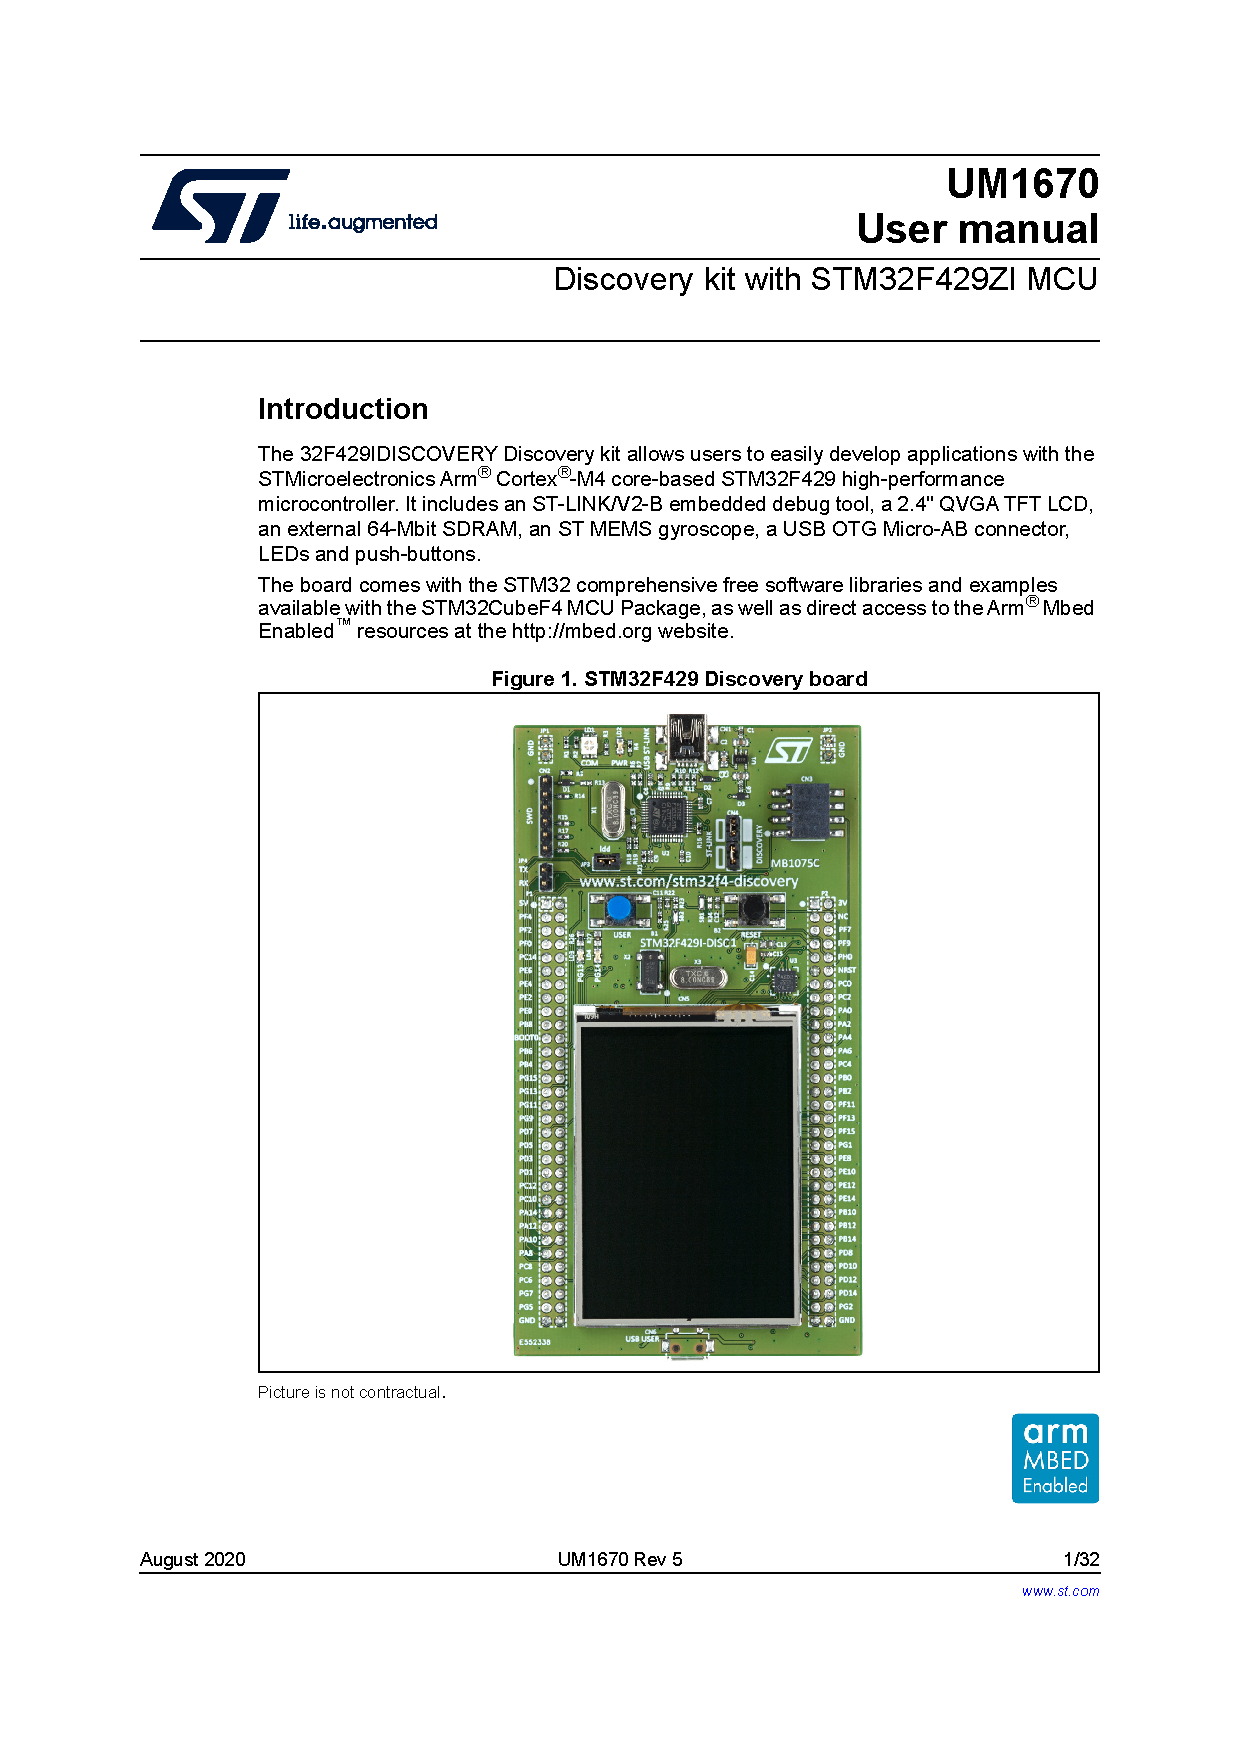
\includepdf[pages=-]{um1670-discovery-kit-with-stm32f429zi-mcu-stmicroelectronics.pdf}


\end{document}
